\documentclass[12pt]{article}

\usepackage{ulem}
\usepackage{float}
\usepackage{graphicx}
\usepackage{fancyhdr}
\usepackage{setspace}
\usepackage[hidelinks]{hyperref}
\usepackage[spanish]{babel}
\usepackage{mlmodern}
\usepackage{longtable}
\usepackage{tabularx}
\usepackage{multicol}
\usepackage[T1]{fontenc}
\usepackage[left=2cm, right=2cm, top=4cm, bottom=2.5cm, headheight=2cm, headsep=1cm]{geometry}
\renewcommand{\normalsize}{\fontsize{13}{15}\selectfont}

\pagestyle{fancy}
\fancyhead[C]
{
    \makebox[\textwidth]{
        \hspace{-0.2\textwidth}
        \begin{minipage}[c][2.5cm]{0.2\textwidth}
            
\includegraphics[width=2.5cm]{logo}
        \end{minipage}
        \hspace{0.01\textwidth}
        \begin{minipage}[c][2.5cm]{0.6\textwidth}
            \centering
            \textbf{\LARGE Colegio Bautista Libertad}\\[0.2cm]
            \textbf{\Large Capacitación docente 2025}\\
            Contacto: soporte@cbl-edu.com
        \end{minipage}
    }
}
\fancyhead[L]{}
\fancyhead[R]{}
\fancyfoot[C]{Pág. \thepage}

\setlength{\parskip}{1.7mm}
\setlength{\parindent}{0pt}

\renewcommand{\headrulewidth}{0pt}

\usepackage{tocloft}
\hypersetup{colorlinks=true,linkcolor=black,urlcolor=blue,citecolor=blue}

\newcommand{\stepTitle}{\par\hspace{2mm}\\\textbf{\large Pasos}\par}
\newcommand{\step}[1]{\par\textbf{Paso #1.}}
\newcommand{\wsm}{\textit{wsmcbl} }
\newcommand{\cbl}{\textit{cbl} }
\newcommand{\quations}[1]{``#1'' }

\begin{document}
    \begin{multicols}{2}
        \textbf{Encuentro:} 2\\
        \textbf{Fecha:} 4 de abril de 2025\\
        \begin{flushright}
            \textbf{Elaborado por:}\\
            Kenny Jordan Tinoco\\
            Ezequiel de Jesús Urbina
        \end{flushright}
    \end{multicols}

    \tableofcontents
    \thispagestyle{fancy}

    \section{Introducción}

    El presente documento expone los casos de usos más importantes de \wsm.

    Este documento aborda los aspectos que el cuerpo docente debe conocer para el uso correcto de
    esta herramienta, se abordan los aspectos de inicio de sesión en el sistema, ver sección guiada, registro de
    calificaciones, historial de calificaciones y navegación entre las distintas las opciones.

    \section{Desarollo}

    En esta sección veremos como interactuar con los casos de usos del sistema.
    Se necesita un dispositivo con accesos a internet, de preferencia una computadora.

    \subsection{Iniciar sesión}

    Para el inicio de sesión se requiere credenciales del usuario, si no las tiene la administración de \cbl se la suministrará.

    \stepTitle

    \step{1} Ingrese a la página oficial de \cbl por medio del enlace \href{www.cbl-edu.com}{cbl-edu.com}.
    \step{2} Diríjase a la parte superior derecha y seleccione la opción \quations{WSM CBL}.
    Esta opción lo llevará hacía \href{wsm.cbl-edu.com}{wsm.cbl-edu.com}.

    \step{3} Ingrese el correo institucional de \cbl y su contraseña. Ver figura 2.
    \step{4} Se ingresa a su perfil en \wsm. Ver figura 3.

    %\begin{figure}[H]
    %    \centering
    %    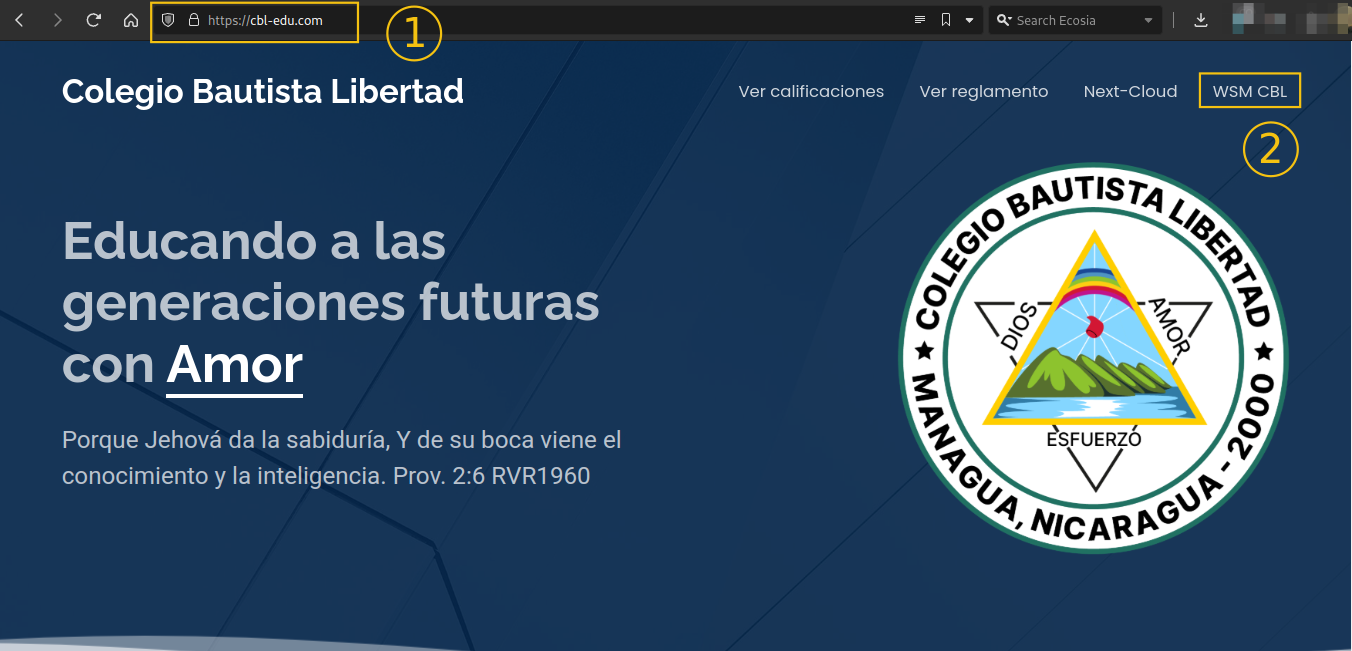
\includegraphics[width=\textwidth]{image/login.01}
    %    \caption{Paso 1 y 2.}
    %    \label{fig:login1}
    %\end{figure}

    \textbf{Nota:} Todo lo realizado en \wsm es parte de la información interna del colegio.
    Esto no será visible al público por medio del sitio web.
    Por tanto, es de suma importancia \textbf{no compartir sus credenciales} con ninguna persona, para salvaguardar la
    integridad de los datos en la institución.

    Si perde sus credenciales recurra a dirección o bien al correo \href{mailto:soporte@cbl-edu.com}{soporte@cbl-edu.com}
    para ayudarle con su caso.

    \subsection{Ver sección guiada}

    El docente necesita conocer la información completa de su sección guiada.
    Para este caso de uso el docente debe tener asignada una sección, en caso contrario esté caso de uso se muestra vacío.

    \stepTitle
    \step{1} Iniciar sesión en el sistema.
    \step{2} Diríjase a la barra lateral izquierda y seleccione la opción \quations{Sección Guiada}.
    \step{3} Se muestra la información de la sección guiada.
    \begin{itemize}
        \item Cantidad de estudiantes.
        \item Cantidad de varones y mujeres.
        \item Capacidad de la sección.
        \item Lista oficial de estudiantes.
        \item Lista de asignaturas y docente correspondiente.
    \end{itemize}



    \subsection{Ver perfil del estudiante}

    El docente necesita conocer la información de cada estudiante en su sección guiada.
    El sistema \wsm registra los datos más importantes en el proceso de matrícula y el docente puede acceder a ella.

    \stepTitle

    \step{1} Iniciar sesión en el sistema.
    \step{2} Ingresar a la ventana de sección guiada.
    \step{3} Elija un estudiante y seleccione los tres puntos en la parte derecha.
    \step{4} Seleccione la opción \quations{Ver perfil}.


    \subsection{Actualizar perfil del estudiante}

    Al inicio de año lectivo se revisa y ajusta la información de cada estudiante para garantizar la integridad de los datos.
    El sistema \wsm permite a los docentes guías actualizar los perfiles de estudiantes en su sección.

    \stepTitle
    \step{1} Iniciar sesión en el sistema.
    \step{2} Ingrese al perfil de un estudiante.
    \step{3} Actualize los datos.
    \step{4} Seleccione \quations{Actualizar datos}.

    \textbf{Nota:} La opción de actualizar perfil de estudiante no está habilitada por defecto.
    Es necesario que dirección autorice y conceda el permiso a los docentes.


    \subsection{Registrar calificaciones}

    Para registrar calificaciones del parcial actual se necesita que esté activa la propiedad \textbf{registro de calificaciones}.
    En caso contrario ninguna calificación se registra en el sistema.
    Sin embargo, las calificaciones ya registradas se visualizan sin necesidad de esta propiedad activada.
    Esto será así para calificaciones del parcial actual o anteriores.

    Cada parcial tiene la propiedad \textbf{registro de calificaciones}.
    Esto es un rango de tiempo en el cual los docentes pueden ingresar y modificar las notas de los estudiantes.
    Este rango puede ser desde \textit{una hora} hasta \textit{quince días}, la duración lo decide dirección.


    \stepTitle
    \step{1} Iniciar sesión en el sistema.
    \step{2} Diríjase a la barra lateral izquierda y seleccione la opción \quations{Calificar}.
    \step{3} Se muestra la lista de secciones del docente.
    \step{4} Elija una sección y seleccione \quations{Ver}.
    \step{5} Se muestra la información de la sección
    \begin{itemize}
        \item Lista de estudiantes ordenados por sexo y nombre.
        \item Lista de asignaturas del docente.
        \item Campos para ingresar las calificaciones.
    \end{itemize}

    \step{6} Ingrese las calificaciones de los estudiantes en cada asignatura.
    \step{7} Ingrese las calificaciones de conducta.
    \step{8} Seleccione guardar.

    \textbf{Importante:} Si el docente imparte más de una asignatura en la misma sección, la calificación de conducta ingresada
    será la conducta para cada asignatura por separado.

    Por ejemplo, si tiene dos asignaturas en la sección y para el estudiante \quations{Jordan Tinoco} la calificación
    de conducta en la tabla es de 89, \wsm internamente registra la conducta de las dos asignaturas como 89.
    Análogamente, sucederá con una cantidad $n$ asignaturas.

    Por otra parte, el docente puede realizar correcciones a las calificaciones ingresadas mientras el registro de
    calificaciones esté activo.
    Si no ingresa las calificaciones de uno o más estudiantes, \wsm establece a cero como calificación por defecto.
    Esto nos da la facilidad de no ingresar todas las calificaciones desde el inicio y realizarlo de manera paulatina.

    \subsection{Ver informe de calificaciones}

    El docente guía necesita conocer el desempeño de los estudiantes en sus distintas asignaturas.
    El sistema \wsm calcula promedios y estadísticas automáticamente, y el docente puede obtenerlos.
    Esto reduce el trabajo que se realiza en cada corte evaluativo.

    \stepTitle
    \step{1} Iniciar sesión en el sistema.
    \step{2} Diríjase a la barra lateral izquierda y seleccione la opción \quations{Informe de calificaciones}.
    \step{3} Se muestra tres pestañas, las cuales muestran los datos referentes al parcial actual.
    \begin{itemize}
        \item Rendimiento: Muestra el promedio de los cuatro parciales para cada estudiante.
        \item Sabana: Muestra el detallado de calificaciones para cada estudiante.
        \item Estadística: Muestra estadísticas mined de estudiantes y calificaciones.
    \end{itemize}

    Estos datos pueden ser solicitados por parcial en cualquier momento, con lo cual es posible realizar un análisis
    de desempeño de los estudiantes.


    \section{Conclusión}

    Debido a la forma de operar del Colegio Bautista Libertad este sistema trata de ser lo menos invasivo con respecto
    a los docentes, con lo cual esta herramienta solo necesita dos aspectos del cuerpo docente; que provea de manera
    íntegra los datos de calificaciones para cada uno de sus estudiantes, y que
    vele por la correcta información de los estudiantes en el sistema.

    Teniendo presente que el éxito que \wsm pueda tener, recaerá en el uso correcto y constante de la información que se
    registre, espera digitalizar y optimizar los procesos internos del Colegio Bautista Libertad con éxito.

\end{document}